\documentclass[fr]{../../../../../../eplexam}

\usepackage{../../../edp-EPL1103-exam}
\usepackage[SIunits]{../../../../../../eplunits}

\hypertitle{Math\'ematique}{3}{FSAB}{1103}{2017}{Janvier}{All}
{Martin Braquet}
{Jean-François Remacle, Grégoire Winckelmans et Roland Keunings}

\section{}
On considère l'EDP suivante
$$ \alpha \:x\:t \: \frac{\partial u}{\partial x}+\frac{\partial u}{\partial t}+\beta \:u=0$$
avec $\alpha$ et $\beta$ des constantes telles que: $\alpha>0$ et $\beta >0$.

On a $0 \leqslant x < \infty$ et $0 \leqslant t < \infty$. De plus, la solution $u$ a pour condition initiale: $u(s,0)=f(s)$ avec:
$$
f(s)=
\left\{
\begin{array}{cl}
u_0\frac{s}{L} & \mbox{si } 0\leqslant s \leqslant L \\
u_0(\frac{L}{s})^2 & \mbox{si } s \geqslant L
\end{array}
\right.
$$
et L est une constante donnée.
\begin{enumerate}
  \item Donnez les unités de $\alpha$ et $\beta$.
  \item Obtenez le réseau de caractéristiques (équation et esquisse). L'esquisse doit être réalisée pour $s=0,L/2$ et $L$, avec des axes adimensionnels (\textbf{Aide}: $e^{1/8}\simeq 1,13$ et $e^{1/2}\simeq 1,65$). Pourquoi ne peut-on pas imposer de condition limite en $x=0$?
  \item Donner la solution $u(x,t)$ pour les 2 morceaux. A partir de quel temps adimensionnel la solution commence-t-elle à croître?
\end{enumerate}

\begin{solution}

On a 
$$ dx=\alpha xt \:dt$$
$$ \int_s^x{\frac{dx'}{x'}}=\alpha \int_0^t{t'dt'}$$
$$ x=se^{\frac{\alpha t^2}{2}}$$
ou 
$$ s=xe^{\frac{-\alpha t^2}{2}}$$
Les caractéristiques issues de $x=0,L/2$ et $L$ sont représentées ci-dessous.
\begin{solfig}{c}{Réseau des caractéristiques}
    \centering
    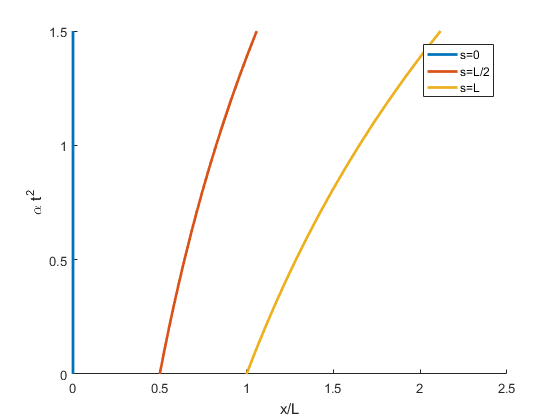
\includegraphics[scale = 0.5]{Math.png}
    %\caption{}
\end{solfig}

La solution ne peut donc pas être donnée en $x=0$ puisqu'elle y est déterminée par la caractéristique issue de l'origine.

On calcule $u$:
$$ Rdt=Qdx$$
$$ -\int_0^t{\beta dt}=\int_{u(s,0)}^{u(x,t)}{\frac{du}{u}}$$
$$ u(x,t)=u(s,0)e^{-\beta t}$$

$$
u(x,t)=
\left\{
\begin{array}{cl}
u_0\frac{s}{L}e^{-\beta t} & \mbox{si } 0\leqslant s \leqslant L \\
u_0(\frac{L}{s})^2e^{-\beta t} & \mbox{si } s \geqslant L
\end{array}
\right.
$$
$$
u(x,t)=
\left\{
\begin{array}{cl}
u_0\frac{x}{L}e^{-\frac{\alpha t^2}{2}-\beta t} & \mbox{si } 0\leqslant s \leqslant L \\
u_0(\frac{L}{x})^2e^{\alpha t^2-\beta t} & \mbox{si } s \geqslant L
\end{array}
\right.
$$

En traçant la solution pour x fixé, on voit bien qu'elle commence à croître pour $\frac{\alpha t}{\beta}=1/2$ et $ s \geqslant L$:\\
\begin{solfig}{c}{Solution $u(t)$ pour différentes valeurs de s}
    \centering
    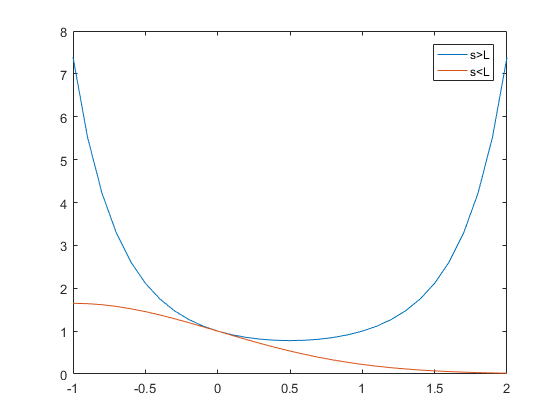
\includegraphics[scale = 0.6]{math2.png}
    %\caption{}
\end{solfig}

Note: on peut le trouver sans Matlab en calculant les racines du polynôme de second degré dans l'exponentielle. Puisque la fonction exponentielle est strictement croissante, elle présente les mêmes variations que son argument. On voit que la première solution pour $s \leqslant L$ n'a pas de racine strictement positive.

\end{solution}

\section{}

On considère l'équation de Laplace
$$\nabla^2 u(r,\theta)=0 $$
sur un secteur d'anneau d'angle d'ouverture $\beta$. Le rayon interne vaut $a$ et le rayon externe vaut $b$.

On a
$$ u(r,0)=0 \qquad u(a,\theta)=0 \qquad u(r,\beta)=u_0\ln(\frac{r}{a}) \qquad \frac{\partial u}{\partial r}(b,\theta)=\frac{u_0}{b}g(\theta)  $$
\begin{enumerate}
\item Faites un dessin du domaine dans le plan (x,y) et (r,$\theta$).
\item Résolvez cette équation par la méthode de séparation de variables en posant 
$$u(r,\theta)=u_p(r,\theta)+u_h(r,\theta)$$ 
où $u_p(r,\theta)$ correspond au mode 0. Écrivez clairement les intégrales à résoudre en fonction de $g(\theta)$.

\textbf{Aide}:
$$ rR''+R'=0  \mbox{ a pour solution } R(r)=C\ln\Big(\frac{r}{L}\Big)+D$$
$$r^2R''+rR'-k^2R=0 \mbox{ a pour solution } R(r)=C\Big(\frac{r}{L}\Big)^k+D\Big(\frac{r}{L}\Big)^{-k}$$

\end{enumerate}

\begin{solution}

Le secteur d'anneau se représente comme ceci:
\begin{center}
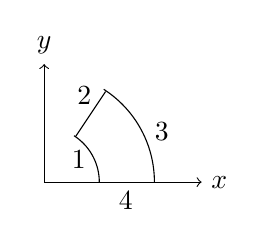
\begin{tikzpicture}
      \draw[->] (0,0) -- (2,0) node[right] {$x$};
      \draw[->] (0,0) -- (0,1.5) node[above] {$y$};
       \put(10, 5){$1$}
       \put(12, 28){$2$}
       \put(40, 15){$3$}
       \put(27, -10){$4$}
      \draw[-] (0.4,0.58) -- (0.78,1.15);
      \draw[scale=0.35,domain=0:1,smooth,variable=\y,black]  plot ({cos(\y r)*2},{sin(\y r)*2 });
      \draw[scale=0.35,domain=0:1,smooth,variable=\y,black]  plot ({cos(\y r)*4},{sin(\y r)*4 });
    \end{tikzpicture}
    \end{center}
Par séparation de variable, on écrit u sous la forme
$$ u(r,\theta) = R(r)\Theta(\theta)$$
On l'introduit dans l'EDP et on obtient
$$ \frac{r^2R^{\prime\prime}+rR^{\prime}}{R}=-\frac{\Theta^{\prime\prime}}{\Theta}=\pm k^2 =\lambda$$
On résout d'abord le mode $\lambda=0$.

Les conditions sur les bords sont
\begin{enumerate}
  \item $u_p(a,\theta)=0$
  \item $u_p(r,\beta)=u_0\ln(\frac{r}{a})$
  \item $\frac{\partial u_p}{\partial r}(b,\theta)=f(\theta)$ (une fonction inconnue)
  \item $u_p(r,0)=0$
\end{enumerate}
La fonction $f(\theta)$ sera déterminée seulement après que l'on connaisse la solution pour ce mode.

On obtient l'équation pour $R$
$$ rR''+R'=0  $$
qui a pour solution
$$R(r)=C\ln\Big(\frac{r}{a}\Big)+D$$
La constante de longueur $a$ est choisie pour simplifier la résolution par après.

Par la condtion sur 1),
$$R(a)=0 \Rightarrow D=0 \Rightarrow R(r)=C\ln\Big(\frac{r}{a}\Big)$$
La solution pour $\theta$ est 
$$\Theta(\theta)=\overline{A}\theta+B$$
et par la condition 4)
$$\Theta(0)=0 \Rightarrow B=0 \Rightarrow \Theta(\theta)=\overline{A}\theta$$
Et ainsi
$$u_p(r,\theta)= A\theta \ln\Big(\frac{r}{a}\Big)$$
en renommant $A=\overline{A} C$.
Sur le bord 2), on a
$$u_p(r,\beta)= u_0 \ln\Big(\frac{r}{a}\Big)$$
$$A\beta \ln\Big(\frac{r}{a}\Big)= u_0 \ln\Big(\frac{r}{a}\Big)$$
$$\Rightarrow A=\frac{u_0}{\beta}$$
On peut maintenant seulement trouver la valeur de $\frac{\partial u_p}{\partial r}$ sur le bord 3),
$$\frac{\partial u_p}{\partial r}(b,\theta)=f(\theta)= \frac{u_0\theta}{\beta b}$$
Attaquons nous maintenant à la solution homogène. Les conditions sur les bords doivent satisfaire  $u_h(b,\theta)=u(b,\theta)-u_p(b,\theta)$.
\begin{enumerate}
  \item $u_h(a,\theta)=0$
  \item $u_h(r,\beta)=0$
  \item $\frac{\partial u_h}{\partial r}(b,\theta)=\frac{u_0}{b}g(\theta)-f(\theta)=\frac{u_0}{b}g(\theta)-\frac{u_0\theta}{\beta b}$
  \item $u_h(r,0)=0$
\end{enumerate}
Au vu des conditions homogènes en $\theta$, on choisit $\lambda=+k^2$.

On obtient pour $R(r)$ l'équation
$$r^2R''+rR'-k^2R=0 $$
qui a pour solution
$$R(r)=C\Big(\frac{r}{a}\Big)^k+D\Big(\frac{r}{a}\Big)^{-k}$$
(Note: les aides données à l'examen doivent souvent être utilisées. Il faudrait s'inquiéter si vous n'en avez pas tenu compte dans votre résolution...)

Par la condition 1), on a 
$$R(a)=0\Rightarrow C+D=0\Rightarrow D=-C $$
$$R(r)=C\Bigg(\Big(\frac{r}{a}\Big)^k-\Big(\frac{r}{a}\Big)^{-k}\Bigg)$$
On résout pour $\Theta(\theta)$
$$\Theta''+k^2\Theta=0 \Rightarrow \Theta(\theta)=A^*\cos(k\theta) + B^* \sin(k\theta)$$
et 
$$ \Theta(0)=0 \Rightarrow A^*=0\Rightarrow \Theta(\theta)=B^* \sin (k\theta)$$
Par la condition sur le bord 2)
$$\Theta(\beta)=0\Rightarrow k_n=\frac{n\pi}{\beta}$$
Une solution est donc
$$u_{h,n}(r,\theta)= E_n \sin (k_n\theta)\Bigg(\Big(\frac{r}{a}\Big)^k-\Big(\frac{r}{a}\Big)^{-k}\Bigg)$$
avec $E_n=B_n^*C$.
Enfin, par la principe de superposition des solutions,
$$u_h(r,\theta)= \sum\limits_{n=1}^\infty E_n \sin (k_n\theta)\Bigg(\Big(\frac{r}{a}\Big)^k-\Big(\frac{r}{a}\Big)^{-k}\Bigg)$$
Il reste la dernière condition sur le bord 4) (la plus compliquée) pour déterminer les $E_n$.
$$\frac{\partial u_h}{\partial r}(b,\theta)=\frac{u_0}{b}g(\theta)-\frac{u_0\theta}{\beta b}$$
$$\sum\limits_{n=1}^\infty E_n\frac{k_n}{a}\Bigg(\Big(\frac{b}{a}\Big)^{k-1}+\Big(\frac{b}{a}\Big)^{-k-1}\Bigg) \sin(k_n\theta)=\frac{u_0}{b}g(\theta)-\frac{u_0\theta}{\beta b}$$
Par othogonalité des fonctions propres
$$\sum\limits_{n=1}^\infty \int^\beta_0\sin(k_n\theta)\sin(k_m\theta)\: d\theta=\int^\beta_0\sin^2(k_m\theta)\:d\theta=\frac{\beta}{2},$$
on a
$$\sum\limits_{n=1}^\infty E_n\frac{k_n}{a}\Bigg(\Big(\frac{b}{a}\Big)^{k-1}+\Big(\frac{b}{a}\Big)^{-k-1}\Bigg)\int^\beta_0 \sin (k_n\theta)\sin(k_m\theta)\:d\theta=\int^\beta_0\Bigg(\frac{u_0}{b}g(\theta)-\frac{u_0\theta}{\beta b}\Bigg)\sin(k_m\theta)\:d\theta$$

$$ E_m\frac{k_n}{a}\Bigg(\Big(\frac{b}{a}\Big)^{k-1}+\Big(\frac{b}{a}\Big)^{-k-1}\Bigg)\frac{\beta}{2}=\frac{u_0}{b}\int^\beta_0\Bigg(g(\theta)-\frac{\theta}{\beta}\Bigg)\sin(k_m\theta)\:d\theta$$
La solution finale est donc
$$u(r,\theta)=u_p(r,\theta)+u_h(r,\theta)$$
$$u(r,\theta)=u_0\frac{\theta}{\beta} \ln\Big(\frac{r}{a}\Big)+\sum\limits_{n=1}^\infty E_n \sin (k_n\theta)\Bigg(\Big(\frac{r}{a}\Big)^k-\Big(\frac{r}{a}\Big)^{-k}\Bigg)$$
avec 
$$k_n=\frac{n\pi}{\beta}$$
et
$$ E_n=\frac{2au_0}{b k_n}\frac{\int^\beta_0\Big(g(\theta)-\frac{\theta}{\beta}\Big)\sin(k_m\theta)\:d\theta}{\Big(\frac{b}{a}\Big)^{k-1}+\Big(\frac{b}{a}\Big)^{-k-1}} $$
Il est utile de vérifier les unités, en sachant que les arguments des fonctions (intégrales, exposants) sont adimensionnels, et des sinus sont en radians.

On constate bien que l'intégrale dans $E_n$ est adimensionnelle et que la première fraction a les unités de $u$ ($u_0$) puisque $k_n$ est aussi adimensionnel.

La solution $u_p$ a aussi les unités de $u$ puisque les angles $\theta$ et $\beta$ s'annulent.

La solution homogène fonctionne tout aussi bien, l'argument du sinus a pour unité des radians, $r/a$ est adimensionnel, et $E_n$ a les unités de $u$.
\begin{solfig}{c}{Solution $u(x,y)$ avec $\beta=\pi/4, a=1, b=2$ et $g(\theta)=4\sin(10\:\theta)$}
    \centering
    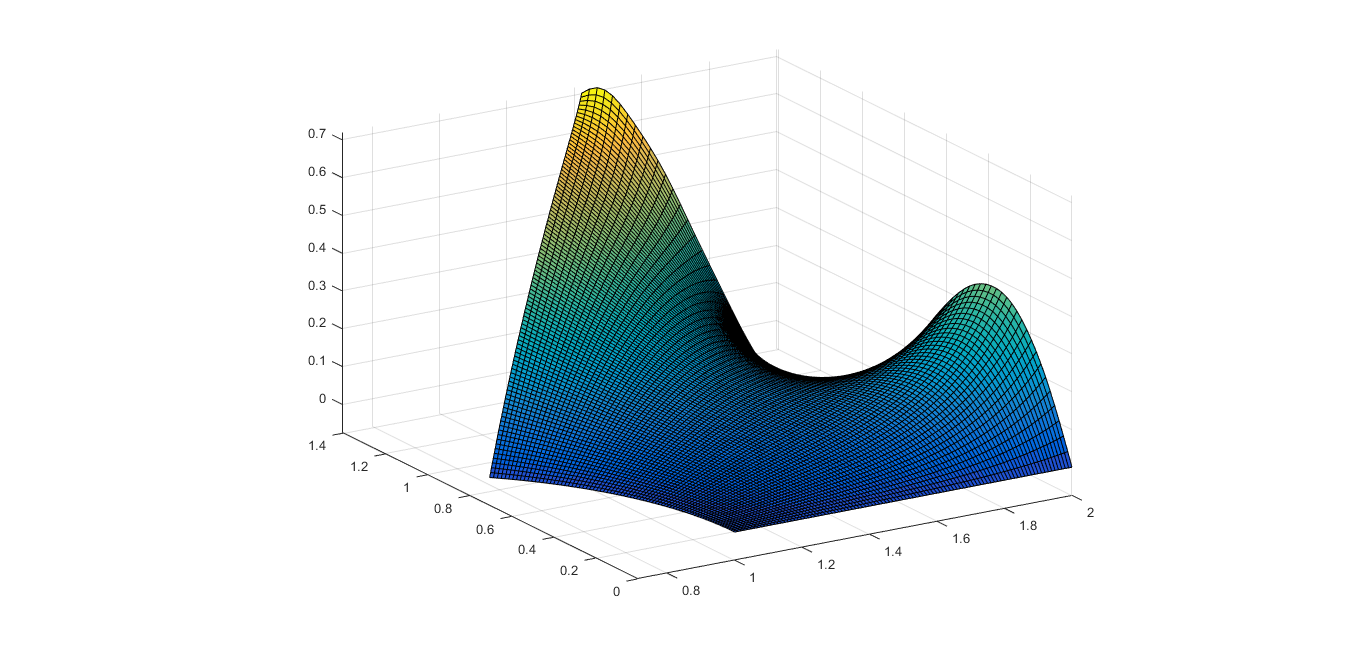
\includegraphics[scale = 0.4]{Math_janvier_2017.png}
    %\caption{}
\end{solfig}

\end{solution}

\section{}
On considère la fonction
$$f(z)=\frac{1}{z\: \sin z}$$
\begin{enumerate}
    \item Montrer que $z=0$ est un pôle $f(z)$. Quel es l'ordre de ce pôle?
    \item Montrer que le résidu de $f(z)$ est nul en ce point.
    \item Quelle conclusion pouvez-vous tirer du point 2 en ce qui concerne le théorème de Cauchy?
\end{enumerate}

\begin{solution}

\begin{description}
\item[Méthode 1] 
\begin{enumerate}
    \item 
On cherche le développement en série de Laurent de $f(z)$. Puisqu'il y a une fonction trigonométrique au dénominateur, la technique consiste d'abord par développer $\sin z$ en série de Taylor autour de 0:
$$\sin z=x-\frac{x^3}{6}+\frac{x^5}{120}+...$$
On pose ensuite
$$f(z)=...+\frac{a_{-3}}{x^3}+\frac{a_{-2}}{x^2}+\frac{a_{-1}}{x}+a_0+a_1x+...$$ qui est le développement en série de Laurent de $f(z)$ autour de 0.

On a donc:
$$\frac{1}{z}=f(z)\sin z$$
$$\frac{1}{z}=a_{-3}\frac{1}{x^2}+
a_{-2}\frac{1}{x}
+(a_{-1}-\frac{a_{-3}}{6})+(a_0-\frac{a_{-2}}{6})x+
(a_1-\frac{a_{-1}}{6}+\frac{a_{-3}}{120})x^2$$
Pour obtenir l'égalité pour tout x, on égale les coefficients des termes de même puissance:
$$
\left\{
\begin{array}{ccc}
0 & = & a_{-3} \\
1 & = & a_{-2}\\
0 & = & a_{-1}-\frac{a_{-3}}{6}\\
0 & = & a_0-\frac{a_{-2}}{6}\\
0 & = & a_1-\frac{a_{-1}}{6}+\frac{a_{-3}}{120}
\end{array}
\right.
$$
On obtient alors
$$
\left\{
\begin{array}{ccc}
a_{-3} & = & 0 \\ 
a_{-2} & = & 1\\ 
a_{-1} & = & 0\\
a_{0} & = & \frac{1}{6}\\
a_{1} & = & 0
\end{array}
\right.
$$
et enfin
$$ f(z)=\frac{1}{z^2}+\frac{1}{6}+... $$
(Note: On voit que l'on pouvait bien se limiter à $a_{-3}$ dans les négatifs puisqu'ils sont tous nuls en dessous de $a_{-2}$)

Le pôle est donc bien d'ordre 2 puisque le premier terme de la série de Laurent est $a_{-2}$.
\item 
Le résidu de $f(z)$ en 0 est donné par le coefficient $a_{-1}$ du terme en $\frac{1}{z}$ de la série de Laurent autour de 0, on a donc $Res(0)=a_{-1}=0$.
\end{enumerate}
\item[Méthode 2]
\begin{enumerate}

\item
On se dit intuitivement que c'est un pôle d'ordre 2 puisqu'il annule "2 fois" le dénominateur: $z$ et $\sin z$.
On pose alors 
$$f(z)=\frac{h(z)}{z^2}\mbox{ et } h(z)=\frac{z}{\sin z}$$
La condition pour obtenir un pôle est
$$h(0)\neq 0 \mbox{ et existe}$$
On vérifie en utilisant l'Hospital
$$h(0)=\frac{0}{\sin 0}\stackrel{\frac{0}{0}}{=}\left.\frac{z'}{\sin'(z)}\right|_{z=0}=\frac{1}{\cos 0}=1$$
C'est donc bien un pôle d'ordre 2.
    \item 
    Le résidu de f(z) en 0 pour un pôle d'ordre 2 est
    $$Res(0)=h'(0)= \left.\frac{\sin z-z \cos z}{\sin^2z}\right|_{z=0}\stackrel{\frac{0}{0}}{=}\left.\frac{\cos z-\cos z+z\sin z}{2\sin z \cos z}\right|_{z=0}
    $$
    $$= \left.\frac{z}{2\cos z}\right|_{z=0}=0$$
\end{enumerate}
\end{description}
3. Le théorème de Cauchy s'énonce

\textit{Soit une fonction $f(z)$ holomorphe sur un domaine D, et C une courbe fermée dans le domaine}, alors 
$$\oint_C f(z)\:dz=0$$
Le point à remarquer est que ce théorème est une implication et non une équivalence. En effet, dans notre fonction, on a
$$\oint_C f(z)\:dz=2\pi i\sum Res(f(z),C)=2\pi iRes(0)=0$$
avec C une courbe fermée entourant l'origine, et puisque 0 est le seul pôle de $f(z)$.

$f(z)$ est donc une fonction \textbf{non holomorphe} sur une domaine D dont l'intégrale sur une courbe fermée de D est nulle!

Finalement,
$$\oint_C f(z)\:dz=0 \nRightarrow f(z) \mbox{ holomorphe sur D}$$

\end{solution}

\section{}
Calculer l'intégrale suivante en utilisant les complexes:
$$\int_{0}^{\infty}{\frac{\sqrt{x}}{(1+x)(2+x)}dx}$$
Note: les 5 lemmes de Jordan sont donnés.

\begin{solution}

On pose
$$f(z)=\frac{\sqrt{z}}{(1+z)(2+z)}$$
On calcule d'abord les pôles: $z=-1$ et $z=-2$. L'origine est un point de branchement, il va donc falloir faire une coupure démarrant de ce point. Puisqu'on doit intégrer sur l'axe réel positif, on choisit une coupure telle que $0\leqslant arg(z) < 2\pi$, le parcours d'intégration va donc passer par cet axe et il ne changera pas de branche lors de son circuit fermé.
On choisit donc un contour d'intégration en trou de serrure pour éviter le point de branchement (\textbf{Remarque}: on ne peut choisir un contour passant par l'axe réel négatif car les pôles sont dessus).

On a alors
$$\int_C{f(z)dz}=2\pi i(Res(-1)+Res(-2))$$
On peut montrer par les lemmes de Jordan que les 2 intégrales sur les cercles de rayon $R->0$ et $\epsilon->0$ sont nulles. Voici la résolution pour le cercle extérieur:
$$0<\lim_{R \to \infty}|f(z)z|=\lim_{R \to \infty}\left|\frac{\sqrt{Re^{i\theta}}}{(1+Re^{i\theta})(2+Re^{i\theta})}Re^{i\theta}\right|$$
$$\leqslant \lim_{R \to \infty}\left|\frac{R^{1/2}e^{i\theta/2}}{(R-1)(R-2)}R\right|=\lim_{R \to \infty}\left|\frac{R^{3/2}}{(R-1)(R-2)}\right|=0 $$
en posant $z=Re^{i\theta}$. L'inégalité de Cauchy est importante pour ce calcul:
$$|z_1+z_2|\geqslant||z_1|-|z_2||$$
Elle permet cela:
$$|1+Re^{i\theta}|\geqslant|1-R|=|R-1|$$
Par un des lemmes de Jordan, on peut alors dire que 
$$\int_{C_2}{f(z)dz}=0$$
si $C_2$ est le cercle extérieur.
On a ensuite (si $z=se^{i(2\pi-\delta)}$ sur l'encoche):
$$\lim_{\delta \to 0}\int_{\infty}^{0}{\frac{s^{1/2}e^{i(2\pi-\delta)/2}}{(1+se^{i(2\pi-\delta)})(2+se^{i(2\pi-\delta)})}e^{i(2\pi-\delta)}ds}=\int_{\infty}^{0}{\frac{s^{1/2}e^{i\pi}}{(1+s)(2+s)}ds}=\int_{0}^{\infty}{\frac{\sqrt{s}}{(1+s)(2+s)}ds}$$
puisqu'on a changé les bornes d'intégration et que $e^{i\pi}=-1$.

On calcule les résidus, $Res(-1)= i$ et $Res(-2)= -i\sqrt{2}$.
Finalement, on trouve
$$\int_C{f(z)dz}=2\int_{0}^{\infty}{\frac{\sqrt{x}}{(1+x)(2+x)}dx}=2\pi(\sqrt{2}-1)$$
$$\int_{0}^{\infty}{\frac{\sqrt{x}}{(1+x)(2+x)}dx}=\pi(\sqrt{2}-1)$$

\end{solution}

\end{document}
